%Créé par Claudine Allen en collaboration avec Jean-Raphaël Carrier
%(Élimination du labo de résistivité des matériaux (IV) à la fin de l'ère JRC + regroupement des labos VI & VII en début de pandémie COVID-19 => renumérotation XI -> IX maintenant)
%Dernière modification JRC: 13 janvier 2014
%Dernière modification CA: 29 novembre 2022
%********************
%ToDo:
% - Essayer de ramener le travail de rétroingénierie sur le système de mesure de l'accélération gravitationnelle en ayant déjà introduit le calcul du temps avec oscillateurs à l'atelier précédent. Je pense diviser le circuit en 3 blocs délimités par des pointillés qui matchent un peu les autres sections du protocole DIY, en partant par la fin : Intro aux circuits logiques rétroactifs -> avec les comparateurs de début de circuit + bascule asynchrone ; Conception du voltmètre -> avec évaluer le résultat d'accélération gravitationnelle à partir de l'oscillateur + compteur (pas de lien conceptuel dans ce cas, juste pcq plus facile/court pour aller avec le voltmètre plus long) ; Construction de portes logiques -> avec les portes NOR ainsi que AND. Il y a deux hics dans tout ça: 1) difficile d'expliquer les portes NOR, AND sans l'info des autres équipes de bascule & oscillateur ; 2) c'est que c'est trop long/redondant de tout le faire en préparation... devrait être fait juste au labo, voir comment exclure de la préparation.
% - Tester le circuit astable avec l'oscillateur de porte NON-OU et rajouter si ça fait encore des attracteurs étrange en simulation... j'en doute. Pourrait aller avec les oscillateurs de l'atelier précédent en remplaçant l'oscillateur à rétroaction qui bouette?
% - Raccourcir en combinant les sections de préparation et déroulement de l'atelier vu que ça répète le début du lab 7 (à recopier au cours 6 aussi). Réviser et ramener les anciens objectifs en renommant "Thématique et objectifs" en voyant si ça ne serait pas mieux de renommer les sous-objectifs en "but à atteindre ou qqch du genre.

\RequirePackage[l2tabu, orthodox]{nag} %Check for obsolete commands
\documentclass[canadien,12pt,oneside,letterpaper]{article}
%
%-----------------------------------------------------
%Loading packages
%
\usepackage[utf8]{inputenc}
\usepackage[T1]{fontenc}
\usepackage[canadien]{babel}
\usepackage{lmodern}
\usepackage{textcomp}
\usepackage{amsmath,amssymb}
\usepackage{siunitx}
\usepackage{xcolor}
\usepackage[colorlinks=true,allcolors=blue]{hyperref}
\usepackage[all]{hypcap}
\usepackage{graphicx}
\usepackage{float}
\usepackage[americanvoltages,americancurrents,siunitx]{circuitikz}
\usetikzlibrary{babel}
\usepackage{caption}
\usepackage{nameref}
\usepackage[letterpaper,headheight=15pt]{geometry}
\usepackage{fancyhdr}
\usepackage{setspace}
%
%----------------------------------------------------
%Other configurations and layout
%
\sisetup{separate-uncertainty}
\captionsetup{font=small,labelfont=bf,margin=0.1\textwidth}
\pagestyle{fancy}
\fancyhf{}
\lhead{\textsl{GPH-2006/PHY-2002~---~Atelier~IX}}
\rhead{\textsl{Page \thepage}}
\setcounter{secnumdepth}{0}
\setlength{\parskip}{1.5ex plus0.5ex minus0.2ex}
%\onehalfspacing
\interfootnotelinepenalty=10000 %To avoid footnotes spreading on several pages.
%
%---------------------------------------------------
%
\title{\textbf{Atelier IX}\\Portes \& circuits logiques\thanks{Auteurs: Claudine Allen, Jean-Raphaël Carrier, Denis Panneton, Daniel Bouffard-Landry \& Jérémie Guilbert.}}
\renewcommand\footnotemark{}
\date{}

\begin{document}

\maketitle \vspace{-15ex}

\section{Thématique}\label{sec:objectifs}
\vspace{-2ex}
La dernière fonction de circuits électroniques, mais non la moindre, abordée dans ce cours est le calcul informatique utilisé entre autres par nos ordinateurs. La fonction d’interrupteur ouvert/fermé du transistor est la clef pour obtenir deux niveaux discrets en tension et ainsi générer un signal numérique binaire permettant des opérations logiques (algèbre de Boole). L’étudiant.e réalisera donc des circuits de portes logiques à partir de transistors. En plus de ces opérations logiques, l’ordinateur doit aussi se rappeler rapidement des états binaires entre chaque opération. On introduit alors la rétroaction entre portes logiques, ici en circuits intégrés, pour obtenir une mémoire volatile très rapide d’accès avec une bascule asynchrone SR. Il s’agit d’une mémoire vive qui se perd lorsque l’alimentation est coupée, à l’opposé des mémoires de stockage non volatil de l’information binaire. 

\section{Lecture préparatoire}
\vspace{-2ex}
\begin{itemize}
\item complément \textit{Introduction aux signaux numériques}
\end{itemize}

% \section{Matériel}

% La réalisation de ce laboratoire requiert l'utilisation de:
% \begin{itemize}
% \item un bloc d'alimentation;
% \item un oscilloscope;
% \item deux résistances de chacune de ces valeurs : 270~$\Omega$, 560~$\Omega$ et 1~k$\Omega$;
% \item une porte NON;
% \item deux diodes électroluminescentes (DEL);
% \item deux portes NON-OU;
% \item trois transistors;
% \item autres composants, selon votre concept de voltmètre;
% \item une plaquette de montage;
% \item un circuit déjà tout monté pour chronométrer la chute d'une bille (partie~1).
% \end{itemize}

\setlength{\parskip}{1ex plus 0.5ex minus 0.2ex}

\section{Préparation}\label{sec:prep}

AVANT la séance d'atelier, écrivez sommairement dans votre cahier de recherche tout ce que vous prévoyez faire au laboratoire pour atteindre les objectifs. N'oubliez pas de calculer toute valeur ou modèle de référence donné en complément aux fins de comparaison à l'expérience. En plus des manipulations expérimentales, des mesures à prendre et de leur analyse, notez aussi les étapes de modélisation, conception et simulation nécessaires. Plusieurs logiciels spécialisés pour l'électronique listés sur le site de cours, dans la section \texttt{Logiciels} de l'onglet \texttt{Matériel didactique}, vous aideront dans cette préparation. En particulier, l'onglet \texttt{Circuits} de \href{https://www.falstad.com/circuit/}{l'application Web de Paul Falstad} contient pratiquement tous les circuits en atelier, montrant directement les comportements idéaux attendus\footnote{Une liste des circuits se trouve \href{https://www.falstad.com/circuit/directions.html}{ici}, mais elle n'est peut-être pas exhaustive.}. 

\section{Partie 1 --- Portes logiques classiques}

L'objectif de cette partie est de réaliser, modifier et comprendre le fonctionnement des portes de la famille logique résistance-transistor (\textit{resistor-transistor logic,} RTL), telle que celle illustrée à la figure~\ref{fig:NOR}.

\begin{figure}[H]
\centering
\begin{circuitikz} \draw
(0,0) node[ground]{} to[Tnpn,n=q1] (0,2) to[short,-*] (5,2) node[right]{$v_{\mathrm{out}}$} to[leDo] (5,0) node[ground]{}
(3,0) node[ground]{} to[Tnpn,n=q2] (3,2) to[R=270~$\Omega$,-o] (3,5) node[above]{$v_{\mathrm{cc}}=5\:\mathrm{V}$}
(-3,1) node[left]{$A$} to[R=560~$\Omega$,o-] (q1.B)
(-3,-2) node[left]{$B$} to[R=560~$\Omega$,o-] (2,-2) to[short] (2,1) to[short] (q2.B); \end{circuitikz}
\caption{Porte logique à identifier. Ses entrées sont les connexions A et B en tension ($v_{\mathrm{cc}}\rightarrow$~1, \textit{ground}~$\rightarrow$~0) et sa sortie est la diode électroluminescente (allumée~$\rightarrow$~1, éteinte~$\rightarrow$~0).}
\label{fig:NOR}
\end{figure}

\subsection{Questions à explorer avec ce circuit}
%Réponses : http://hyperphysics.phy-astr.gsu.edu/hbase/Electronic/trangate.html , Circuits->Logic families->RTL sur https://www.falstad.com/circuit/ et Resistor–transistor logic (RTL) dans Wikipedia, etc.
\begin{itemize}
    \item Quelle table de vérité obtenez-vous? À quelle porte correspond-elle? %porte NON-OU
    \item Comment pouvez-vous fabriquer une porte NON, \textit{i.e.} un inverseur, à l'aide d'un transistor et de résistances? Quelle est la porte obtenue en ajoutant cet inverseur en sortie du circuit? %porte OU
    \item En refaisant la même porte avec des circuits intégrés sur puce, obtenez-vous de meilleures performances? %Ça devrait pas, avec la beauté du numérique affranchissant du bruit direct, ça devient plutôt des probabilités de causer une erreur computationnelle -> Bit error rate
    \item Est-ce que vous placeriez les transistors en série ou en parallèle pour obtenir une porte NON-ET?
    %\item efficacité énergétique écologique DD avec TTL vs RTL familles de logique "The obvious disadvantage of RTL is its high current dissipation when the transistor conducts to overdrive the output biasing resistor. This requires that more current be supplied to and heat be removed from RTL circuits. In contrast, TTL circuits minimize both of these requirements."; "The evolution of TTL came from efforts to increase transition speed, noise margin, reduce power, while retaining backward-compatibility, input thresholds, fanout=10, output levels." sauf c'est pas tant clair tout ça à partir des designs sur Falstad/Circuits... smaller footprint of transistor compared to resistors, dans complément graphes de taille->densité de transistors par puce pour rapidité mais densité de puissance dissipée pas loin de celle à la surface du soleil!!!! vrai même avec meilleurs CMOS transistors : "Two important characteristics of CMOS devices are high noise immunity and low static power consumption.[3] Since one transistor of the MOSFET pair is always off, the series combination draws significant power only momentarily during switching between on and off states. Consequently, CMOS devices do not produce as much waste heat as other forms of logic, like NMOS logic or transistor–transistor logic (TTL), which normally have some standing current even when not changing state. These characteristics allow CMOS to integrate a high density of logic functions on a chip. It was primarily for this reason that CMOS became the most widely used technology to be implemented in VLSI chips." de https://en.wikipedia.org/wiki/CMOS
\end{itemize}
 

\section{Partie 2 --- Circuit logique rétroactif}
L'objectif ici est de démontrer en pratique que la bascule $SR$, représentée à la figure~\ref{fig:RS-latch}, a une mémoire pouvant être utilisée dans un calcul.

\begin{figure}[h]
\centering
\begin{circuitikz} \draw
(0,2) node[nor port](norR){}
(norR.in 1) to[short] (-1.5,2.28) node[left]{$R$}
(norR.in 2) to[short] (-2.5,1.72) to[short] (-2.5,-1) to[short] (0.5,-1) to[short] (0.5,0)
(norR.out) to[short] (1,2) node[right]{$Q$}
(0,0) node[nor port](norS){}
(norS.in 1) to[short] (-1.5,0.28) to[short] (-1.5,0.5) to[short] (0.5,1.75) to[short] (0.5,2)
(norS.in 2) to[short] (-1.5,-0.28) node[left]{$S$}
(norS.out) to[short] (1,0) node[right]{$\overline{Q}$}
;\end{circuitikz}
\caption{Circuit bistable, \textit{i.e.} ayant deux états stables en sortie complémentaire $Q$ et $\overline{Q}$, qui est une bascule asynchrone sur les entrées $S$ et $R$ en tension.}
\label{fig:RS-latch}
\end{figure}

\subsection{Questions à explorer avec ce circuit}
\begin{itemize}
    \item Quels sont les fils qui créent la rétroaction?
    \item Comment pouvez-vous tester le fonctionnement de cette bascule? Est-ce qu'il correspond à celui décrit en complément?
    \item Pourquoi ce circuit a-t-il une mémoire?
    \item Que se passe-t-il si vous utilisez les sorties $Q$ et $\overline{Q}$ en entrée d'une porte NON-OU?%Ça devient mêlant, plutôt remplacer par une porte NON-ET? Je pensais aller même vers implémenter l'opération d'addition binaire https://en.wikipedia.org/wiki/Adder_(electronics), mais ça devient rapidement compliqué.
\end{itemize}

\section{Partie 3 --- Conversion analogique-numérique}

L'objectif final de cet atelier est de réaliser une conversion analogique-numérique, explorant ainsi le principe au cœur du module d'acquisition qui vous a permis de mesurer des tensions à l'ordinateur dès le début du cours. Parmi les nombreux types de conversions possibles, c'est la conception d'un convertisseur direct qui est demandée en utilisant seulement une source d'alimentation DC, des ampli-ops, des résistances identiques et des diodes électroluminescentes (DELs). L'affichage en sortie doit se faire dans le système de numérotation unaire, d'où le convertisseur agira comme un voltmètre en base 1 avec un changement d'affichage numérique à chaque incrément de 1~V.

%Réaliser une conversion analogique-numérique en base 1 à l'aide d'un circuit simple. Ce circuit est en fait un embryon de voltmètre à concevoir à partir d'une source d'alimentation DC, de la fonction comparateur d'ampli-ops, de résistances identiques et de diodes électroluminescentes (DEL). Ces dernières afficheront la valeur d'un signal de tension dans le système de numérotation unaire, ce signal étant fourni par un générateur de fonctions ou autre source variable. Plus précisément, \textbf{aucune} DEL ne doit s'allumer lorsque la tension est inférieure à 1~V, \textbf{une} DEL doit s'allumer lorsque la tension fournie est supérieure à 1~V et \textbf{deux} DEL doivent s'allumer lorsque la tension devient supérieure à 2~V.

% Voir si j'inclus l'image de convertisseur analogique numérique 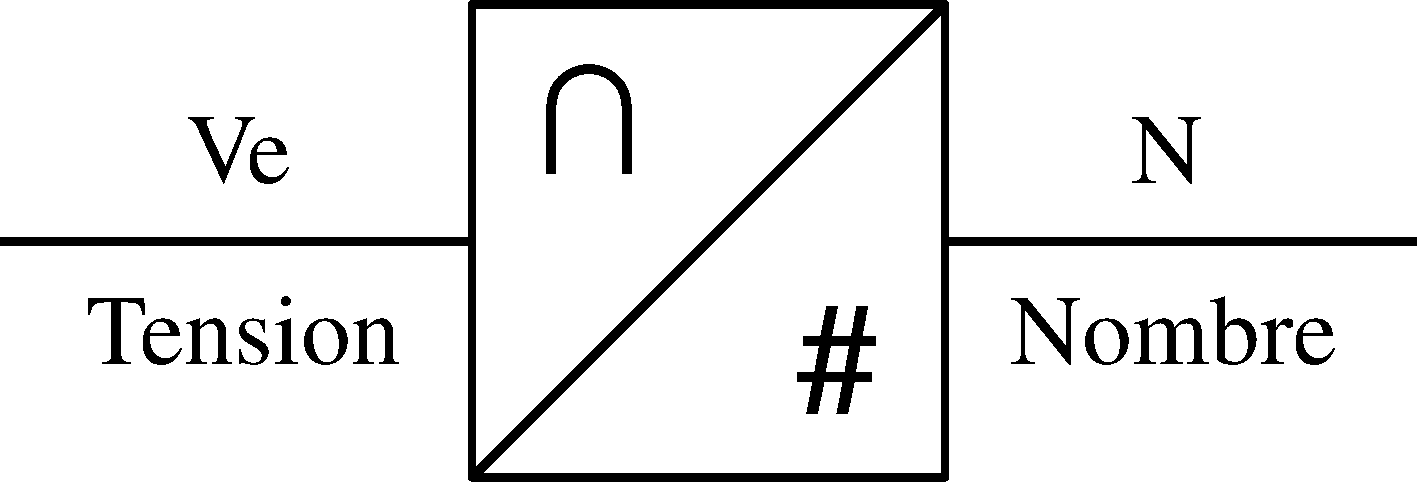
\includegraphics[width=0.5\textwidth]{ADC_symbol.png} Citation : Par Jacques.boudier — Travail personnel, CC BY-SA 3.0, https://commons.wikimedia.org/w/index.php?curid=27303393

\subsection{Pistes à explorer}
\begin{itemize}
    \item Revoir la liste des fonctions électroniques étudiées dans ce cours, fournie en accompagnement du projet de conception, pour identifier celles réalisables avec les composants électroniques imposés. %diviseur de tension, comparateur
    \item Rechercher des exemples de convertisseurs analogique-numérique (\textit{Analog-to-digital converter,} ADC) en ligne, sans oublier notre \href{https://www.bibl.ulaval.ca}{bibliothèque universitaire} qui garantit la crédibilité des ressources cataloguées.
    \item Faire un diagramme schématique du circuit et les calculs théoriques associés pour le modèle idéal de convertisseur sélectionné.
    \item Vérifier ses calculs en simulant ce circuit à l'aide de votre app préférée de la section \texttt{Matériel didactique} $\rightarrow$ \texttt{Logiciels} sur le site de cours.
    \item Tester le fonctionnement de conversion avec un signal à mesurer connu en entrées parallèles du circuit.
\end{itemize}
%Ça serait sympa si c'est digeste et pas trop long d'ajouter l'encodeur de https://en.wikipedia.org/wiki/Flash_ADC

\section{Partie 4 optionnelle --- Portes logiques quantiques}

Je change de style d'écriture (C.A. au clavier), ne sachant plus si je devrais rajouter cette introduction à l'informatique quantique dans l'atelier en considérant la charge de travail de l'ensemble du cours. Je croyais pertinent d'inclure ce nouveau domaine en intense développement technologique grâce à la physique et pour ce faire, j'ai coupé une partie de l'atelier qui découvrait le fonctionnement d'un circuit logique inconnu pour mesurer l'accélération gravitationnelle. Ceci dit, c'est peut-être trop lourd à ajouter puisque je dois introduire une nouvelle série de concepts associée à la superposition d'états quantiques et le qubit qui en découle. Bref, je sollicite votre opinion à ce sujet idéalement via le questionnaire mentionné dans la section \nameref{sec:pedago}, qui regroupe les rétroactions sur le cours, mais je lirai aussi tout courriel qui me sera envoyé à ce sujet par la suite.

Si vous avez le temps et l'intérêt, explorez le matériel didactique listé ci-dessous qui est proposé par les entreprises qui se sont lancées ou associées à la construction d'ordinateurs quantiques accessibles à distance. Laissez-moi savoir quel est le contenu pédagogique qui vous interpelle le plus et sur lequel je devrais me baser pour bonifier cet atelier s'il y a lieu.

\begin{itemize}
    \item Les \href{https://pennylane.ai/qml/quantum-computing}{introductions}, \href{https://pennylane.ai/codebook}{codebook} et \href{https://docs.pennylane.ai/en/stable/}{documentation} de Pennylane
    \item \href{https://learning.quantum.ibm.com/catalog/courses}{IBM Quantum Learning}
    \item Les ressources éducatives de \href{https://quantumai.google/resources}{Google Quantum AI}
    \item Le centre de formation de \href{https://www.quandela.com/products-and-services/training-center/}{Quandela} dont l'approche expérimentale est la plus près de mon propre Laboratoire d'optique de la matière condensée (labOMC).
\end{itemize}


\section{Partie 5 --- Pédagogie}\label{sec:pedago}

Le deux derniers objectifs du cours sont :

\begin{itemize}
    \item de vous rendre sur le site Web du cours dans la section \texttt{Évaluations et résultats} pour les ateliers et y évaluer vos pairs sur leur contribution respective au travail du groupe,
    \item prendre le temps de remplir le questionnaire d'appréciation de l'enseignement avec des critiques constructives, aussi précises que possible. Toutes les suggestions d'amélioration sont les bienvenues! Si vous n'avez pas reçu le lien de ce questionnaire dans un courriel signé par le Service de soutien à l’enseignement, veuillez nous en aviser svp.
\end{itemize}

%%%%MOT DE LA FIN SUR MICROPROCESSEURS -> Arduino donc projet, FRONTIÈRE INFORMATIQUE/ÉLECTRONIQUE.

\end{document}

% \begin{figure}[h]
% \centering
% \begin{circuitikz} \draw
% (7,1) node[ground]{} to[Tnpn,n=q3] (7,3) to[R=270~$\Omega$,-o] (7,6) node[above]{$v_{\mathrm{cc}}$}
% (0,0) node[ground]{} to[Tnpn,n=q1] (0,2) to[short] (3.5,2) to[R=500~$\Omega$] (q3.B)
% (3,0) node[ground]{} to[Tnpn,n=q2] (3,2) to[R=270~$\Omega$,-o] (3,5) node[above]{$v_{\mathrm{cc}}$}
% (-3,1) node[left]{$A$} to[R=560~$\Omega$,o-] (q1.B)
% (-3,-2) node[left]{$B$} to[R=560~$\Omega$,o-] (2,-2) to[short] (2,1) to[short] (q2.B)
% (7,3) to[short,-*] (9,3) node[right]{$v_{\mathrm{out}}=A+B$} to[leDo] (9,1) node[ground]{}
% ;\end{circuitikz}
% \caption{Circuit interne simplifié d'une porte OU créée en ajoutant une porte NON à la sortie d'une porte NON-OU.}
% \label{sch-OR}
% \end{figure}